\begin{textarea}[]
  \only<1>{
    \centering
    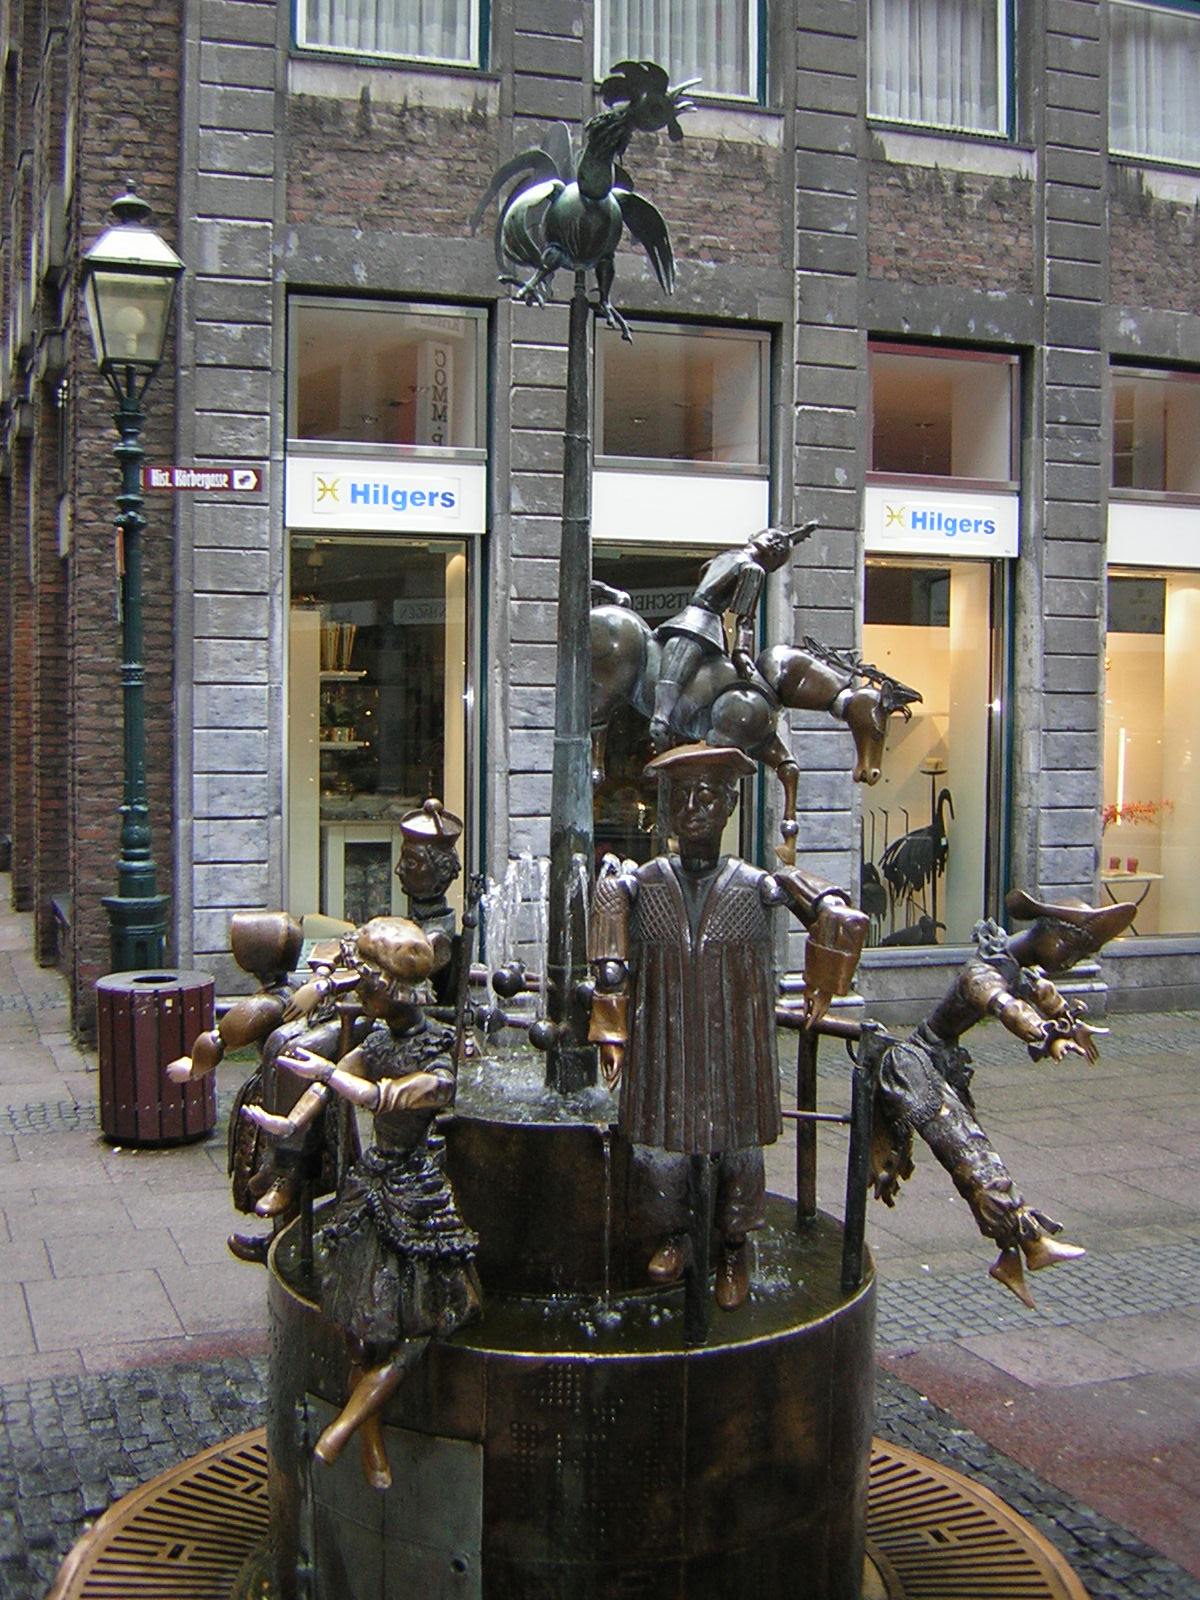
\includegraphics[height=0.5\linewidth]{categories/media/Puppenbrunnen_in_Aachen.JPG}
  }
  \only<2>{
    What is the Puppenbrunnen?
  }
\end{textarea}

\begin{textarea}[]
  \only<1>{
    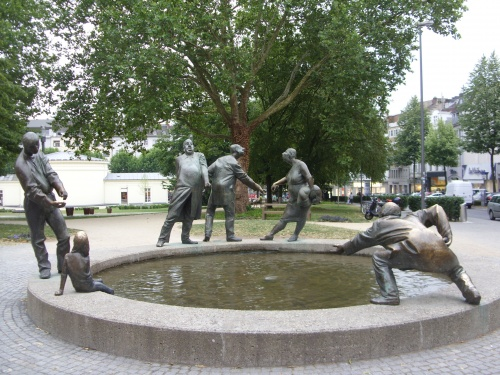
\includegraphics[height=0.5\linewidth]{categories/media/LaufDesGeldes}
  }
  \only<2>{
    What is Kreislauf des Geldes?
  }
\end{textarea}


\begin{textarea}[]
  \only<1>{
    \begin{columns}[c] 
      \column{.5\textwidth} 
      \includegraphics[height=1.0\linewidth]{categories/media/Löwenstein_House_Aachen}
      \column{.5\textwidth}
      It is one of Aachen's oldest buildings and can be found on the market square.
    \end{columns}

  }
  \only<2>{
    What is L\"owenstein house?
  }
\end{textarea}

\begin{textarea}[]
  \only<1>{
    \centering
    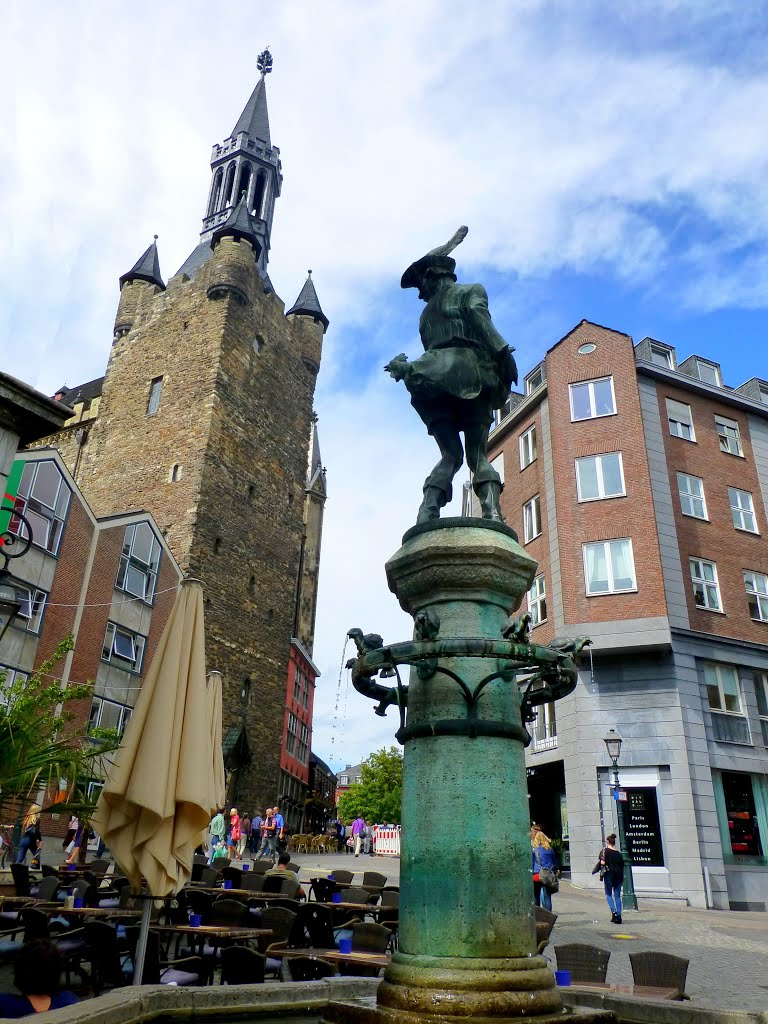
\includegraphics[height=0.5\linewidth]{categories/media/huehnerdieb}
  }
  \only<2>{
    What is the H\"uhnerdieb?
  }
\end{textarea}

\begin{textarea}[]
  \only<1>{
    \begin{columns}[c] 
      \column{.5\textwidth} 
      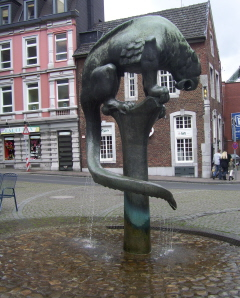
\includegraphics[height=1.0\linewidth]{categories/media/Brunnen-am-buechel}
      \column{.5\textwidth}
      It is the monster of an Aachen legend, which drunk husbands used as an excuse to come home late.
    \end{columns}
  }
  \only<2>{
    What is the Bahkauv?
  }
\end{textarea}

\begin{textarea}[]
  \only<1>{
    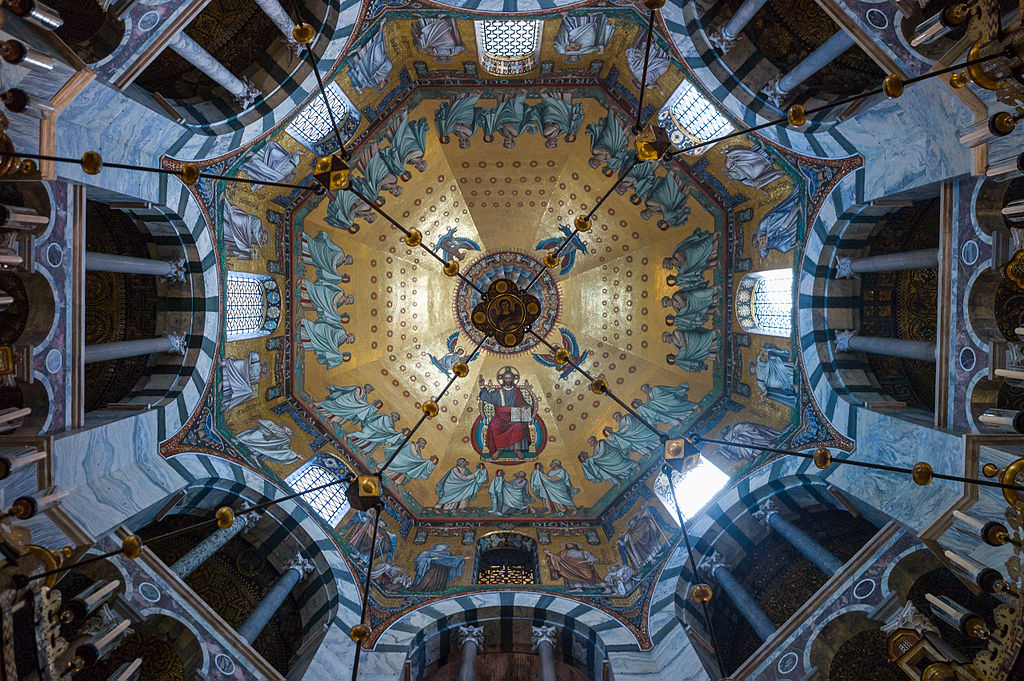
\includegraphics[height=0.5\linewidth]{categories/media/Aachener_Dom_August_2014}
  }
  \only<2>{
    What is Aachen cathedral?
  }
\end{textarea}

\begin{textarea}[]
  \only<1>{
    \begin{columns}[c] 
      \column{.5\textwidth} 
      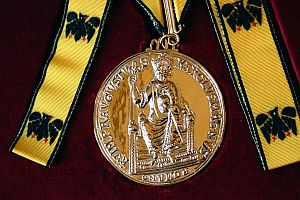
\includegraphics[height=0.5\linewidth]{categories/media/CharlemagnePrize}
      \column{.5\textwidth}
      Parts of this building date back to Charlemagne, who can be seen on the prize that is rewarded in this building once a year.
    \end{columns}
  }
  \only<2>{
    What is Aachen Town Hall?
  }
\end{textarea}

